\section{Discrete Adjoint Solutions based on a Primal Problem}
\label{section:Discrete_Adjoint}
\subsection{Background}

Following the adjoint formulation explained in section \ref{section:Adjoint} it is seen that the adjoint formulation (also known as the \textit{dual problem}) can be written as a linear system:

\begin{equation}
A^Tx = -b^T
\end{equation}

Thus we can write the transpose of the Residual Jacobian matrix, $\frac{\partial{R}}{\partial{U}}$ as matrix $A^T$ and the right hand side vector b as the derivative of the functional with respect to the state,$\frac{\partial{J}}{\partial{U_i}}$\par

Some current plots obtained for the adjoint sensitivities are shown in figure \ref{fig:Adjoints}. The initial condition was that of a shock cube problem, and average pressure was selected as the functional, $J$. This case is still ongoing as the formulation is still being verified.\par

\begin{figure}[t!]
  \centering
	\subfigure[Initial conditions with large density and pressure jumps between left and right states]
   {\label{fig:init_cond}	   
   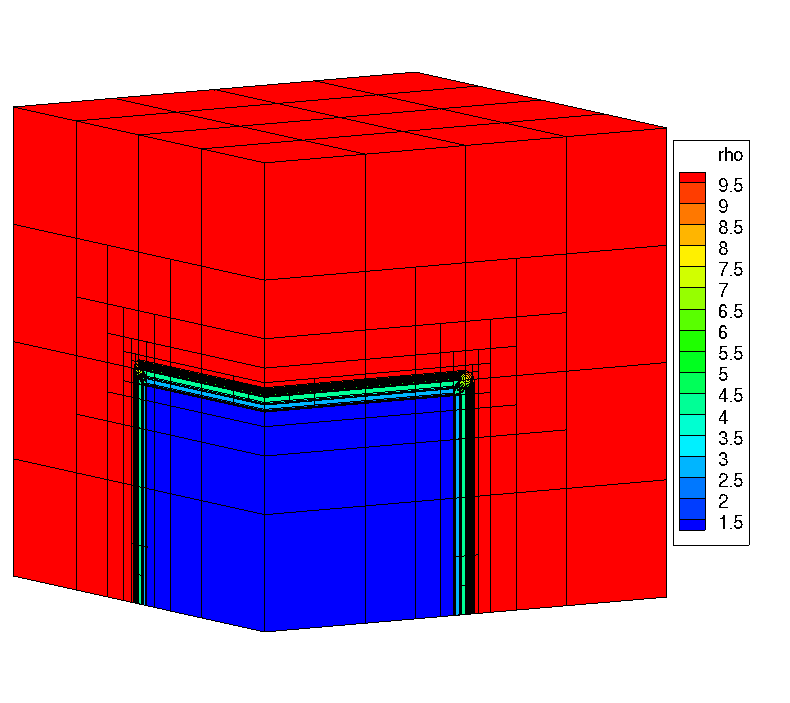
\includegraphics[height=0.3\textwidth, trim=0.2cm 0.2cm 0.2cm .2cm,clip=true]{figs/shockCubeAll1.png}}%
   \:
   \subfigure[sensitivity to Density]
   {\label{fig:rho_Adjoint}	   
   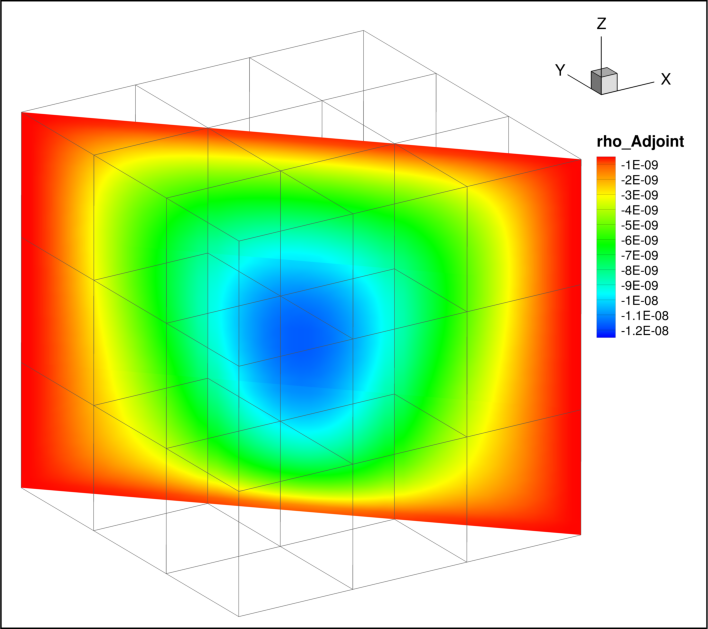
\includegraphics[height=0.3\textwidth, trim=0.2cm 0.2cm 0.2cm .2cm,clip=true]{figs/rho_Adjoint.png}}%
	\:
	\subfigure[sensitivity to x-Momentum]
   {\label{fig:u_Adjoint}	   
   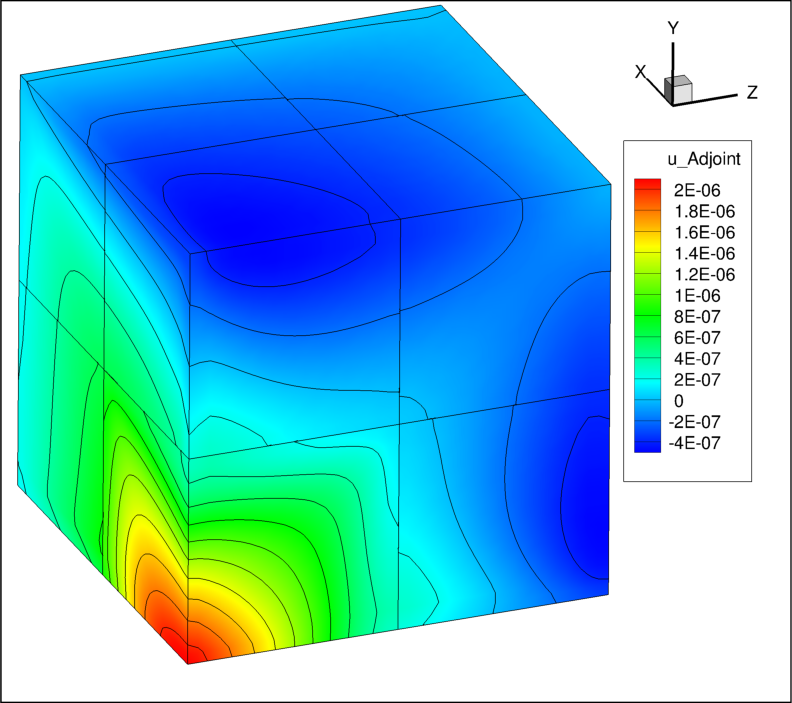
\includegraphics[height=0.3\textwidth, trim=0.2cm 0.2cm 0.2cm .2cm,clip=true]{figs/u_Adjoint.png}}%
   \:
	\subfigure[sensitivity to Pressure]
   {\label{fig:p_Adjoint}	   
   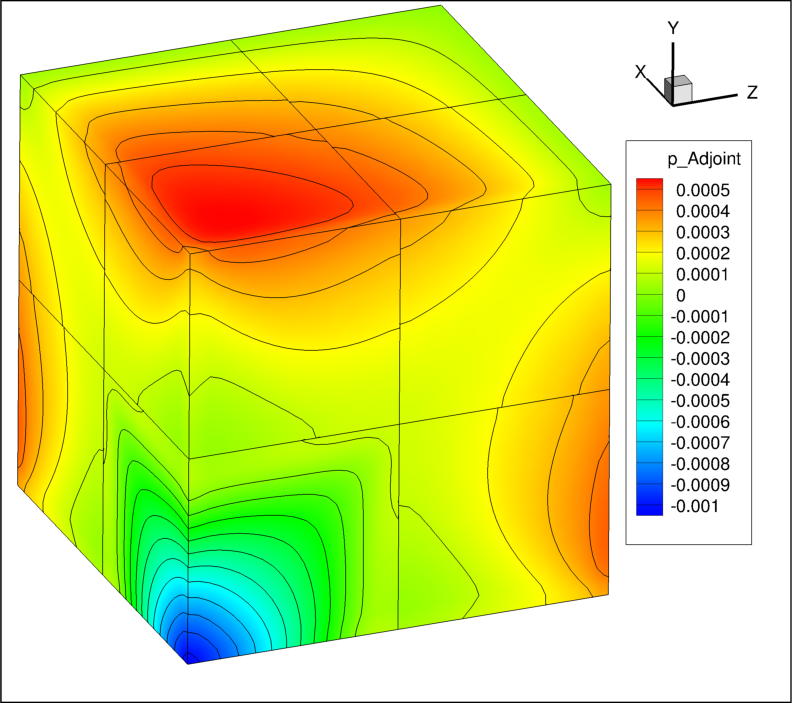
\includegraphics[height=0.3\textwidth, trim=0.2cm 0.2cm 0.2cm .2cm,clip=true]{figs/p_Adjoint.png}}%
   \caption{Contours of adjoint sensitivities to changes in the conserved state variables } 
\label{fig:Adjoints}      
\end{figure}  